\newpage
\parindent=1cm %красная строка? 
\begin{center}
	\addcontentsline{toc}{section}{Введение} %Убираем номер , даём имя в оглавлении 
	\section*{Введение} %сам текст заголовка 
	\pagestyle{plain} % нумерация выкл.
	\setcounter{page}{3} % начать нумерацию с номера тр
\end{center}

В настоящее время на рынке информационных технологий представлено множество средств защиты личных и корпоративных данных. Однако, средства проведения информационных атак  развиваются  быстрее, чем имеющиеся средства защиты, таким образом создавая <<черный>>  рынок с вредоносным программным обеспечением  и множеством разнообразных математических и социальных  алгоритмов проведения атак. 

Анализ инцидентов информационной безопасности, проведенный в конце 2016 года международной компанией <<Positive Technologies>> показал, что в 2017 ожидается на 30\% больше инцидентов по информационной безопасности в финансовой сфере и появление новых, более убедительных средств социальной инженерии.\cite{AntiMail1} %LITER : https://www.anti-malware.ru/analytics/Threats_Analysis/Analysis_information_security_threats_2016_2017  
%GRAPH Распределение типов атак, применяемых злоумышленниками, AntiMailware https://www.anti-malware.ru/analytics/Threats_Analysis/Analysis_information_security_threats_2016_2017
\begin{figure*}[h!]
	\centering{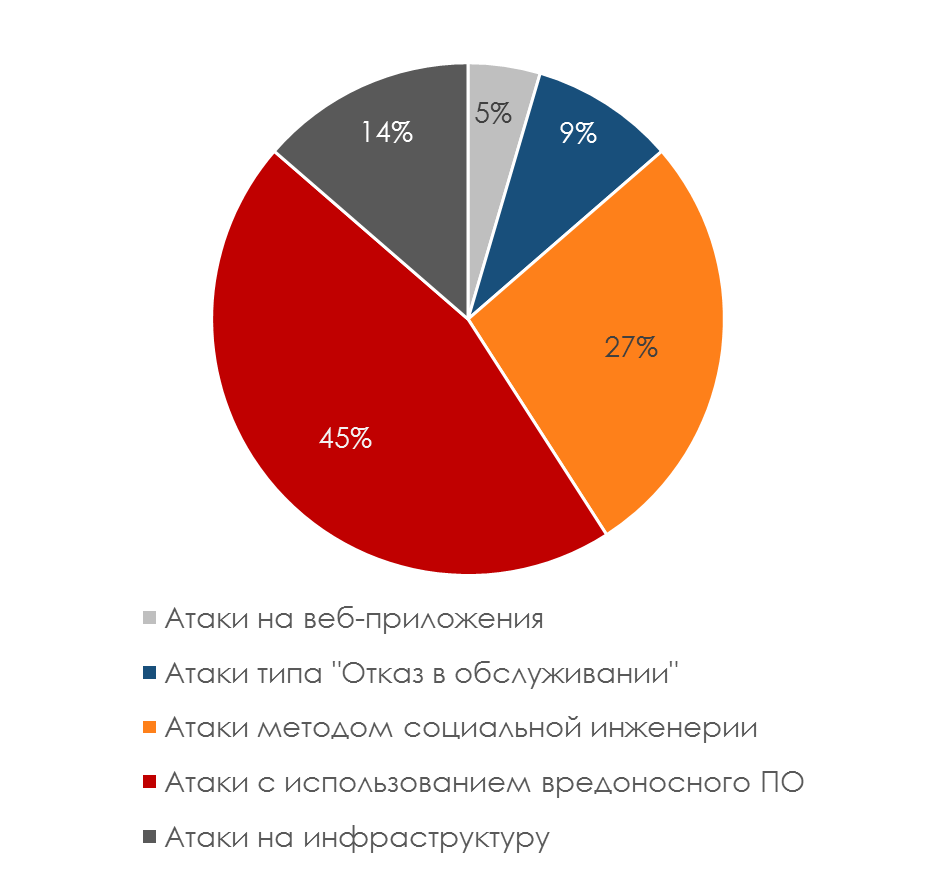
\includegraphics[scale=0.8]{AntiMail.png}}
	\caption{ Распределение типов атак, применяемых злоумышленниками в 2016-2017 годах по данным портала AntiMailware \cite{AntiMail1}}.
\end{figure*} 
Также, исследования  <<Angara Technologies Group>> 
показывают, что многие сотрудники  как частного, так и государственного сектора слабо информированы и обучены правилам обращения с данными внутри организаций, что приводит к растущему числу утечек организационных и личных данных по аналоговым (физическим)  и цифровым (информационным) каналам.  Кроме очевидного,  сложно измеримого вреда деловой репутации, отмечаются  более понятные негативные последствия утечек — отмена сделок, компенсация ущерба третьим лицам, затраты на судопроизводство \cite{AntiMail2}. %LITER :https://www.anti-malware.ru/analytics/Threats_Analysis/main-channels-information-leakage-in-enterprise

Исходя из данных результатов исследований и прогнозов, можно сделать вывод о необходимости развития социальных  и алгоритмических  методов защиты личных данных, в том числе защиты тайн переписки и  связи.   

\textbf{Актуальность} работы  связана с возросшим числом новых угроз в области защиты личных данных, участившимися атаками частных лиц, группировок и специальных ведомств иностранных государств против частных лиц с целью получения частной информации, анализа полученных личных данных   и использования для шантажа атакуемых лиц, продажи или другого выгодного обмена, а также  в иных противозаконных целях. Данная курсовая работа может быть актуальна в рамках изучения дисциплин связанных с защитой данных и программирования на факультетах математики и информатики, практическая часть работы представляющая собой несколько криптографических алгоритмов вместе с их реализацией может быть использована для изучения современных промышленных языков и технологий программирования (С\#, .Net 4.5). Полученная в результате анализа угроз информация применима для защиты   данных, особенно переписки, частных лиц в общественных и частных сетях. Также, разработанные рекомендации и реализации алгоритмов могут быть применены частными лицами и предприятиями, государственными структурами, в том числе на коммерческой основе. 

\textbf{Целью} данной работы является %EDIT: сделать это в виде списка с пунктами?
 анализ новых цифровых угроз, возникших в последнее десятилетие в связи с бурным развитием информационных технологий, за которым не последовал соразмерный рост знаний пользователей цифровых систем, используемые кибер-преступниками методы анализа и атаки на частные данные, строгое определение понятий <<тайна связи, цифровые угрозы>>, правовой аспект защиты личной переписки и тайны связи, способы борьбы с угрозами  в рамках существующего программного обеспечения, %EDIT: заменить на ПО и создать список используемых сокращений до введения?
 сравнительный анализ существующих продуктов, разработка и реализация собственных алгоритмов для сохранения тайны связи, разработка собственного ПО для зашиты тайны связи.	
 
 В качестве \textbf{объектов исследования} выбраны цифровые данные частных лиц в приватных и организационных сетях, в первую очередь сама  переписка и сведения об абонентах, то есть участниках переписки.
 
 \textbf{Предмет исследования}: изучение методов атак на частные данные, причины утечек этих данных, цели, преследуемые злоумышленниками при проведении атак на частные данные и переписку. Предметы выбраны  с целью создания математических и социальных алгоритмов защиты частных данных и переписки, разработки собственного ПО для охранения тайны связи.
 \newpage %перевод следующей главы на новую страницу с изменеием номера страницы в оглавлении 
